\section{Design}

\todo{High level overview of system}

\begin{figure}
    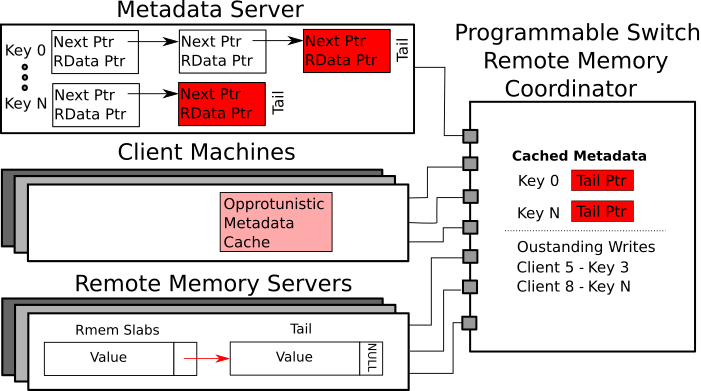
\includegraphics[width=0.45\textwidth]{fig/overview_2.png}
%%
    \caption{ System overview, Metadata, client, and Remote Memory
    servers are Clover components. Our remote memory coordinator is
    located on a centralized TOR interconnecting the clover components.
    }
%%
    \label{fig:overview} 
\end{figure}

\begin{figure}
    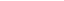
\includegraphics[width=0.45\textwidth]{fig/system.png}
    \caption{Our packet processing pipeline}
    \label{fig:system}
\end{figure}


\subsection{Operation Caching}
\label{sec:operation-caching}

Any asyncronous data structure which allows for lockless reads and writes must
have a mechanism in place to resolve conflicts. When memory is close, conflict
resolution stratatges can make many reads and writes quickly in the uncommon
case of a conflict, the cost of which is typically amortized by the unlikelyhood
of the conflict itself. In the case of far memory the cost of a conflict is
severe. In contrast to opprotunistic algorithms in a shared cache archetecure,
in a disaggretated system with small amounts of in network compute conflicts can
be detected and resolved in the data path. Our solution is to provide a general
framework in which developers with knowledge of their remote structures can
resolve their conflicts in network as the operations flow by serially to memory. 

\begin{figure}
    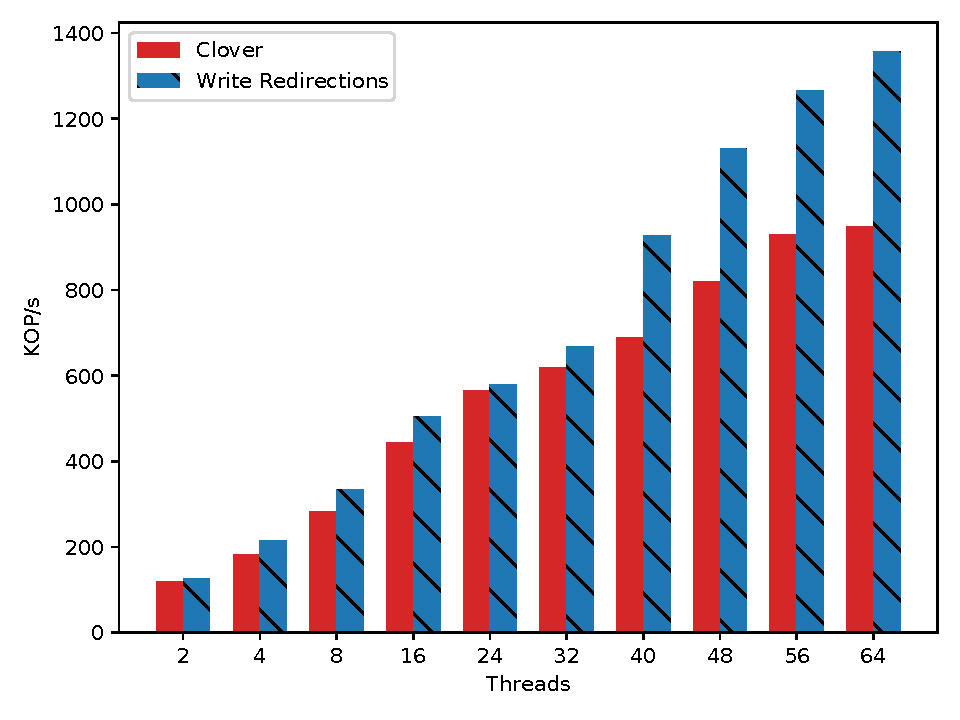
\includegraphics[width=0.45\textwidth]{fig/throughput.pdf}
    \caption{Default Clover throughput vs. Clover with write conflict
    detection and correction turned on \todo{recompute with the read caching values (old)}}
    \label{fig:throughput}
    \vskip -1em
\end{figure}

\textbf{writes:} In the case of clover we cache the location of the latest writes to occur for
each key. If a write occurs which is for a stale virtual address, our conflict
detection algorithm first uses information about clovers algorithm to find the
value of the key in each RDMA write packet. We find this value by checking the
size of the write, and checking the location in the packet for specific clover
data. Once the key from the write is extracted a table lookup is used to
translate the key into the virtual address of the latest write for that key.
This strategy uses 64 bytes per key, as each RDMA virtual address is 64 bytes.
By performing this lookup in the data path all writes succeed reguardless of how
contested the memory address is. ~\ref{figure from words}.

\textbf{reads:} Reads present a slightly more complicated case. Writes contain
the key, which allows for a table lookup, while RDMA read requests only contain
a virtual address and a size. When a read fails it must be retried, as mentioned
earlier reads are performed itterativly untill the tail of the list is reached,
which in the case of highly contested keys could be arbetrarily long. Repeating
reads does not destroy system performance as they are lockless, however in terms
of client latency each retry adds serious latency. What makes handling reads
hard is identifying the clover key for which the read is for, without additional
data in the packet the value must be determined another way. As reads can be for
arbetrarily old virtual addresses a naieve solution would be to store the entire
lineage of each key, which would require caching all of clovers meta data in the
network. Our solution is to hash the address of each write into an array
~\todo{2x} the size of the keyspace. When writes occur their virutal address and
key value are stored in the array. New writes simply overwrite old values in the
table. This allows keys with higher hit rates to maintain longer histories in
the table. When reads occur their address is looked up in the table, if the
address has a hit the read is steered to the tail of the list. If a miss occurs
the read is left to flow through, clovers default mechanism kicks in and
performs a lookup to the meta data server for the last known address and the
process repeats. We found that by using an array size of 8x the ~\todo{vast
majority of reads succeed first try.} While the number of reads that require a
second try is ~\todo{a number}. ~\todo{insert the CDF of read retries}.

\begin{figure}
    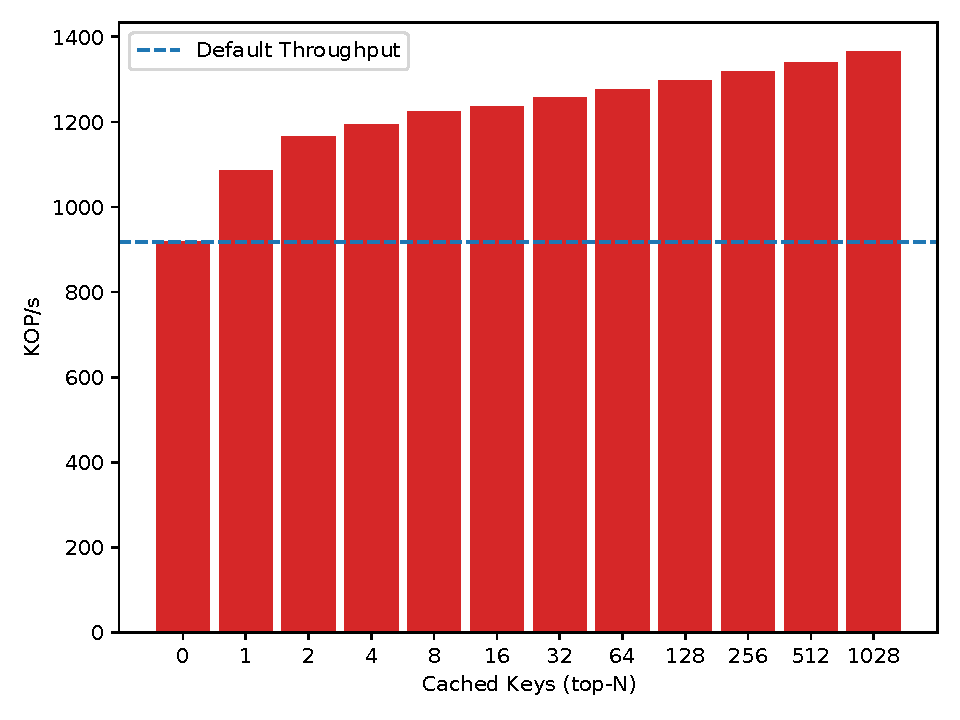
\includegraphics[width=0.45\textwidth]{fig/cache.pdf}
    \caption{Performance as a function of keys cached. Caching a few
    of the top-$N$ keys provides the greatest marginal throughput
    benefits.}
    \label{fig:cache}
\end{figure}

\textbf{reduced cache size} we show that if hot keys are known we require only a
small amount of in netowrk state~\ref{fig:cache} we have considered dynamic
approaches such as LRU which would allows for a finite amount of space and an
arbetrary number of keys to be serviced.

\subsection{Atomic Replacement} Atomic operations are expensive, as such we
would like to replace atomic operations such as CNS with non-blocking operations
such as read and write. Using a middle box the trasnformation is simple, RoceV2
CNS headers are very close to write headers, conceptually its a special case
where the write is conditional and only requires 8 bytes of writing, so swapping
CNS out with write headers can be done inplace while processing a packet. When
the ACK transits back from the memory server, it can be replaced by an atomic
ACK with the original data from the write location filled in by the middle box.
Doing this does nothing to disturb the higher level protocol, as the receiving
NIC processes the requests as is, and the sender gets back the responses it
expects. however all of the safty of the atomic operation is lost.  In the
following subsections we describe the dangers of removing atomics, and present
our solutions.

A few assumptions must be made in order for this repacement of operations to be
made. First and foremost all operation serialization must be made, and finalized
at the point where the CNS is swapped out. More formally, all of the data
structure invariants which required locking, must be satisfied at the time of
transforming the packet. Further the order of operations must be maintained
downstream from the checking of the invariant. These two requirements influence
the design of any system which aims to make this performance improvement. 

\textbf{1) metadata required} The first requirement, that the structural invariants
of the datastructure be maintained at the point of transformation demands that
all of the state required to check the structural invariant be present at the
point in the network at which the swap is made. This fact increases the memory
cost on a switch, however with inteligent data structure design the cost of the
required metadata can be mittigated. In the case of Clover, while each key has
an entire linked list history that can potentially span megabytes, the only
required metadata to make the change from CNS to write is the location of the
tail pointer. In this case the metadata cost is O(n) as it grows linearly with
the keyspace.

\textbf{2) reordering} The second requirement, that operations not be reordered
after the invariant has been checked requires more care in real systems. For
instance in an RDMA system with two clients, both could have contesting CNS
operations swaped with writes. As the two clients are transmitting operations on
separate QP, and the receving NIC makes no guarantees about ordering between QP,
the operations could easily be reordered. In the case with CNS, the order could
be forced by ensuring that if one write was to succeed the second would fail.
Without this guarantee the preservation of operation ordering must be maintained
in another way.

\subsection{Connection Remapping}

While removing locking operations is a general principle here we consider a
solution for RDMA. Different transports with different ordering guarantees would
require bespoke solutions. RDMA ensures that operations performed on the same QP
arrive in order~\cite{infiniband spec}~\footnote{while IB allows for relaxed
ordering here we rely on that feature being turned off on the receiver}. Our
solution is to map all operations for the same shared state to the same QP to
ensure ordering of operations in the absense of locks. Similar to TCP, RDMA RC
ensures that all operations arrive in order. RDMA retransmits requests if
reordering occurs using a go back n algorithm.

Our solution here is simple, given that we have the key's for reads and writes
~\ref{operation-caching}, all operations for the same key are mapped to the same
QP. Doing so requires care on the middlebox. Multiplexing requests onto a single
connection means that the sequence numbers of memory operations must be updated
so that the receiving NIC on the memory side sees monotonic sequence numbers. To
achieve this we track a sequence number per QP and inject the updated sequence
number into the packet after a mapping decision has been made. When a response
comes back (in the form of an ACK, READ RESPONSE, or ATOMIC ACK) the packet must
me demuliplexed back onto it's original connection. In addition to sequence
numbers, a \textit{message sequence number}, is maintained on the recever NIC
for each inbound connection, this value is transmitted as part of the ROCE BTH+
header in the response. It's value corresponds to the highest request number the
receiver has processed. If this value is wrong in the response packet from the
perspective of the sender, the packet is retransmitted. We calculate the message
sequence number a sender expects to see by counting the number of operations a
sender has issued and adding it to the value of the original message sequence
number for that connection. When requests are mutiplexed the QP and sequence
number of the original request are stored in a per QP table. The sequence number
of the response packet is used to perform an O(1) lookup for the original QP and
sequence number.

This algorithm requires that a few pieces of state be maintained per connection.
First the sending and response QP for each sender and receiver need to be
tracked. Second the sequence number of each connection, and the original message
sequence number offset must be maintained. Per client connection the pair of
QP's require 48 bits, and the sequence + message sequence require an additional
48 for a total of 12 bytes per connection. The storage requirement for mapped
requests varies based on the algorithm. If clients are able to issue an
unbounded number of async requests, then a buffer large enough to maintain
backwards mappings for each request is required. In clover clients can issue up
to 2 async requests, so we keep a two 6 byte mappings for each connection
available to map back. 

Depending on the algorithm and the QP mapping scheme requests from a single
sender can be reordered. That is, if a client makes a read and write request to
different locations in memory, and they are mapped to different QP, they may be
returned out of order. Infiniband allows for out of order operations on
receivers~\cite{ib specification}, which pushes operation ordering to client
side user space. Roce does not allow for out of order operations. In this case
the receiving NIC will retransmit if requests are delivered out of order. Here
we buffer requests in network, as we have application knowledge the size of the
buffer is bounded (to the size of a single read packet in clovers case). We
suggest that given the tight memory restrictions on middleboxes algorithms which
have an unbounded number of async requests leave the ordering of remapped
requests to client side user space using IB verbs or a different transport layer
entirely.

\subsection{Instruction Coalescing} A final additional challenge in mapping
requests, is that receving NIC's can coalese acknoledgement messages. Given a
single connection, if two concurrent writes are issued, it is perfectly valid
for an RDMA NIC to only ack the second write. This is a challange when mapping
requests as a coalesed message might have been for a different sender. In our
scheme as all requests have mapping stubs stored in the middle box, when a
request is coalessed a gap in the sequence number is observable. In this case we
generate the coalesed request. While read, and CNS requests can not be
coalessed, CNS requests mapped to writes can be. In the case of coalesed ATOMIC
acks an atomic ACK is generated in place of the coalessed write ack.

\todo{these sections may not be nessisary}

\subsection{Traffic Identification} Depending on the design of a disaggregated
rack memory traffic might be coresident with regular network traffic.
Additionally some of the traffic on the memory bus may not require tracking or
manipulation. In the case of clover we do not modify any traffic to the metadata
server as it is not in the read/write path. The first stage of our packet
processing pipeline is to match requests for manipulation. In our design users
submit a filter as part of their program to allow traffic which does not need to
be modified to flow freely.

\subsection{Dynamic enable/disable of connections, and epochs} A key goal in our
design is to not require the existence of a middle box in the data structures
algorithm. Clover for instance is designed to deal with memory operations made
to the wrong location via iterative pointer chasing. We strongly suggest that
disaggregated algorithms take this approach as our middlebox solution only acts
to acclerate operations in the common case. We add and subtract connections
based on the send and receipt of a single CNS operation. The QP and sequence
number for the CNS are stored on send, and the ATOMIC ACK is used to retreive
the other recevers QP. As this approach requires only a single packet requests
can be added and removed from our algorithm dynamically with little effort. As
some state may be dependent on the number of connections (such as the key to QP
mappings), state transitions either require a lock, or the coping of current
state over to a new epoch when new connections are added. In all of our
experiments only one such transition is made. We begin our mapping after a
specific number of clients for the experiment have connected. Once the total
number of clients have connected, a switch is flipped, and the QP multiplexing
algorithm begins. Requests which do not have mappings stored, but were in flight
during the flip have their sequence numbers, and MSN values applied to the
connection state of the new epoch.

